\section{Задание 2. Обзор интерфейса Ubuntu.}

\subsection{Пункт 1}

Представить рабочий стол Ubuntu, объяснить основные элементы интерфейса, таких как панель задач, меню приложений и другие.

\textbf{Ответ:}

Рабочий стол Ubuntu \ref{fig:desktopUbuntu} :

\begin{figure}[!h]
    \centering
    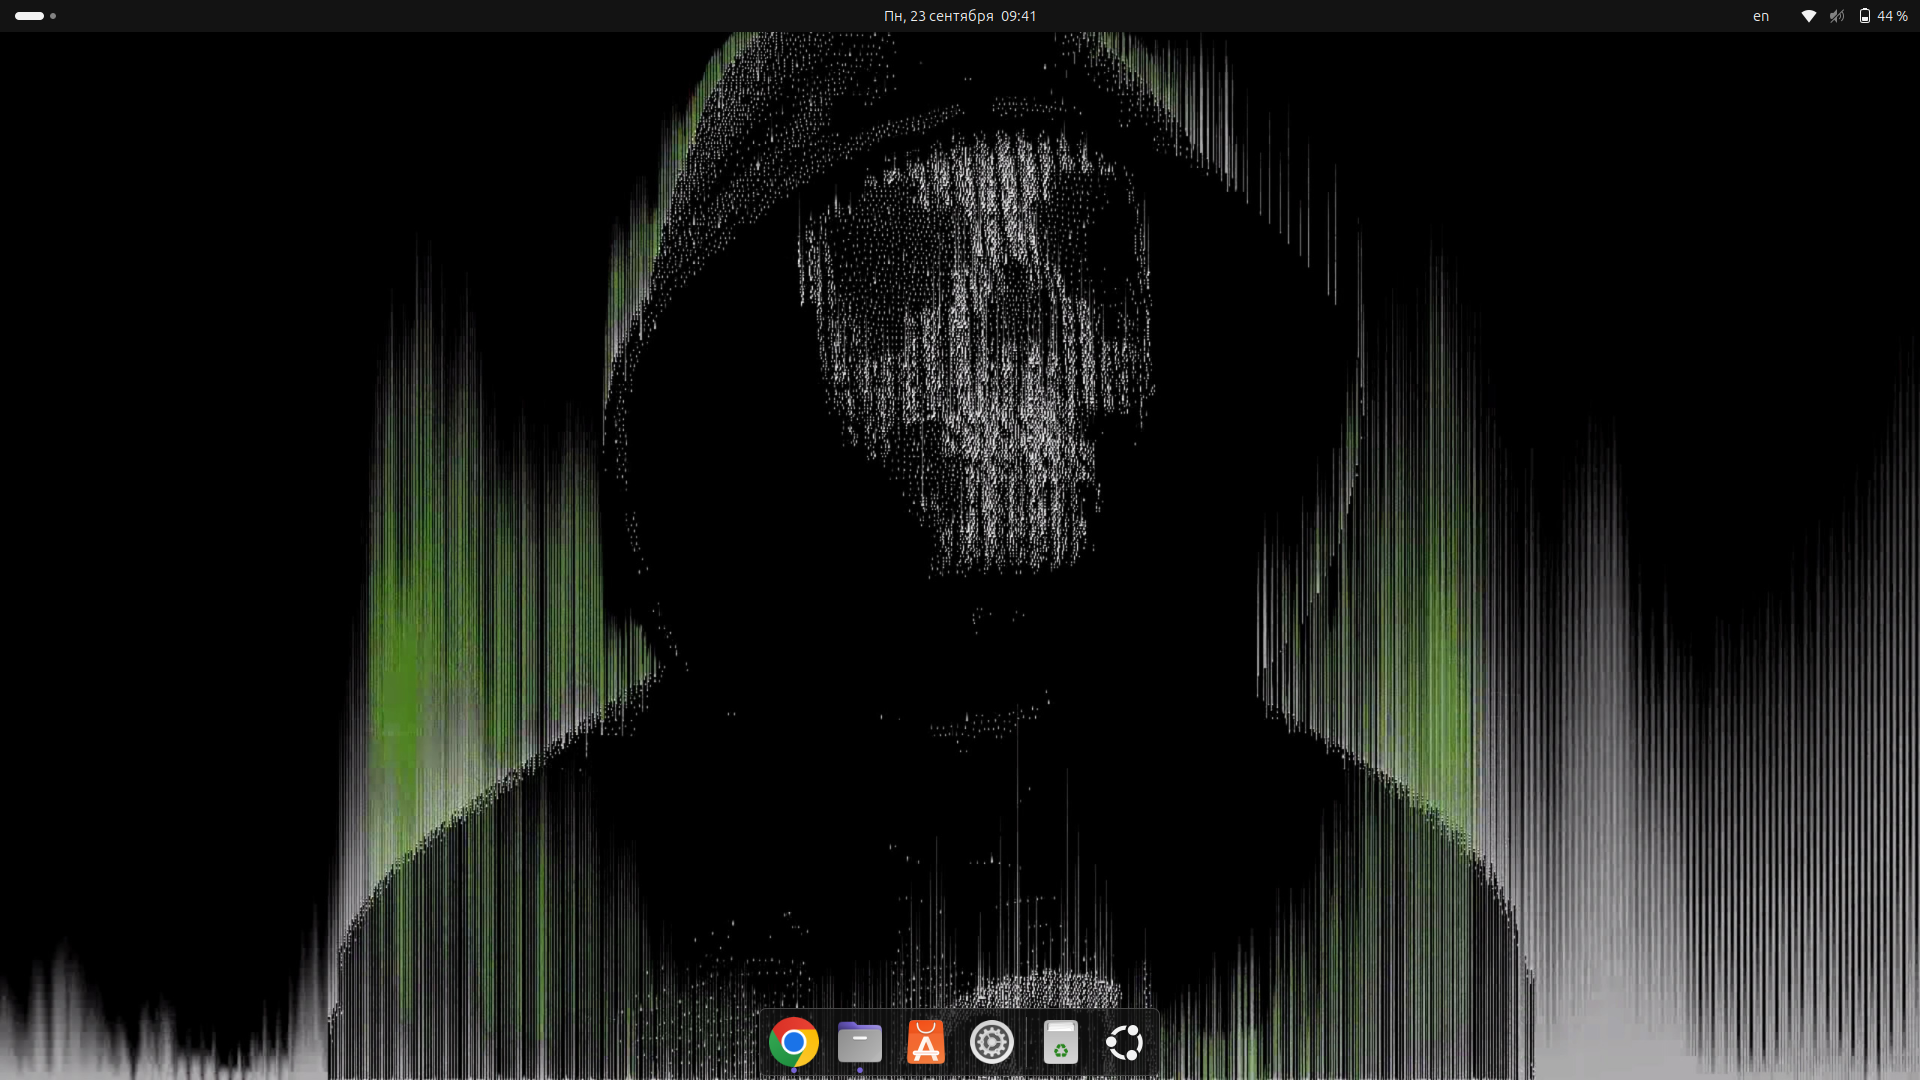
\includegraphics[width = 0.8\textwidth]{images/desktopUbuntu.png}
    
    \caption{Рабочий стол Ubuntu}
    
    \label{fig:desktopUbuntu}
\end{figure}

Панель задач \ref{fig:taskPanel} :

\begin{figure}[!h]
    \centering
    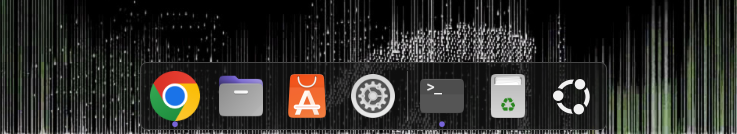
\includegraphics[width = 0.8\textwidth]{images/taskPanel.png}
    
    \caption{Панель задач}
    
    \label{fig:taskPanel}
\end{figure}


Меню приложений \ref{fig:menuApplications} :

\begin{figure}[!h]
    \centering
    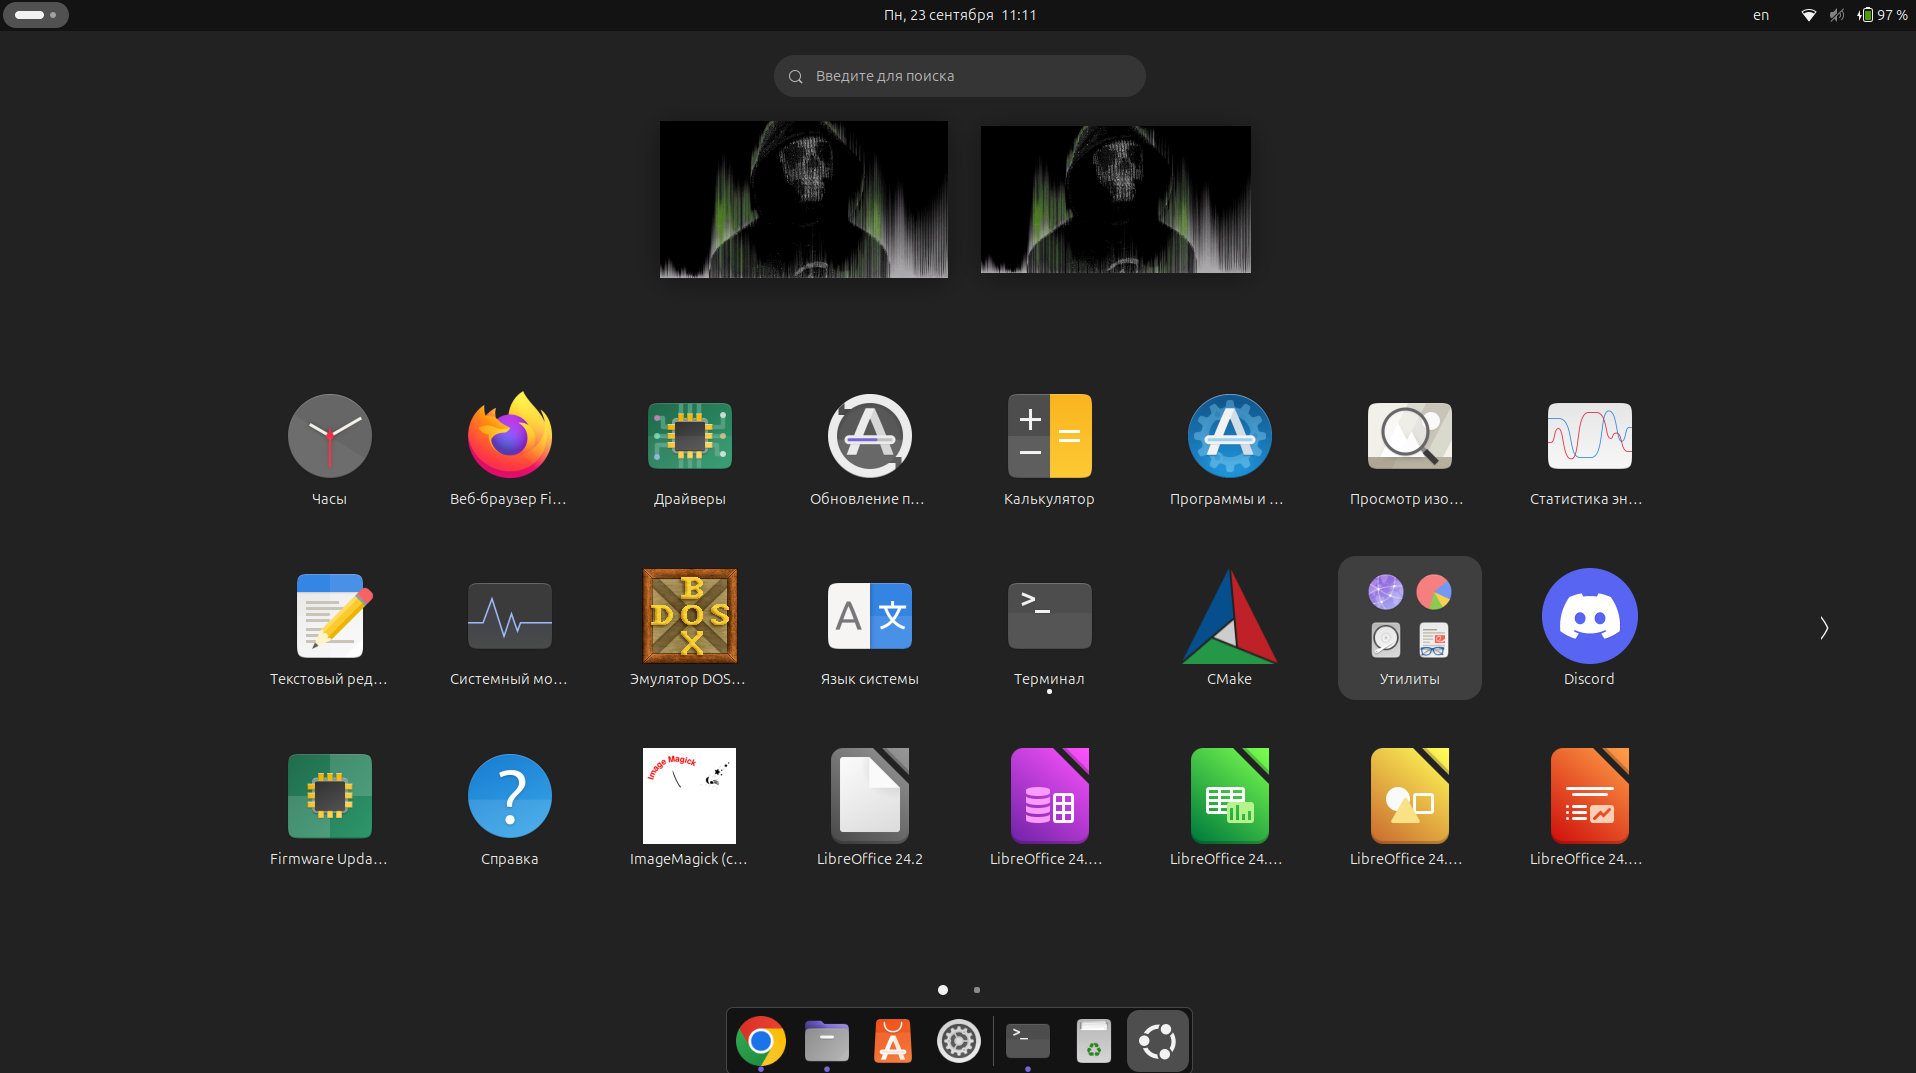
\includegraphics[width = 0.8\textwidth]{images/menuApplications.png}
    
    \caption{Меню приложений}
    
    \label{fig:menuApplications}
\end{figure}
